\subsection{An at-the-money observation from a fitted smile}\label{sec:smileextension}
The within-chain errors need not be inherited by the calendar fit. We now fit a smile to each chain and use its interpolated at-the-money (ATM) price as the observation. An ATM smile estimate supplies a local variance proxy without integrating unobserved tails. It uses the same 555 standard chains and strike screen as the baseline.

Write the terminal futures-index displacement, in rate bp, as a mixture
\begin{equation}\label{eq:mixture}
I_S-I_0\ \sim\ \tfrac12 N(d,s_1^2)+\tfrac12 N(-d,s_2^2).
\end{equation}
The mean is fixed at the observed future. Each component has an elementary normal call formula, and their average gives a convex European price curve. Fit $d,s_1,s_2$ by unweighted least squares to the selected out-of-the-money settlements. Appendix~\ref{app:empiricalmethod} specifies bounds, starts, and convergence checks. The mixture is a price interpolant: it is not asserted to be the terminal law of the Gaussian rate model or a joint model across expiries.

Let $\widehat c_{\rm ATM}$ be its fitted ATM price and define
\begin{equation}\label{eq:smileatm}
\widehat{\cV}_{\rm ATM}=2\pi(\widehat c_{\rm ATM}/D)^2.
\end{equation}
This is the variance giving the same ATM premium in the normal formula. It is generally different from the mixture's second moment $d^2+(s_1^2+s_2^2)/2$. We apply the calendar matrix to this ATM proxy; its additivity is assessed in Section~\ref{sec:additivity}. For a sensitivity allowance $\varepsilon$ around the fitted ATM price, its interval is
\[
2\pi\{(\widehat c_{\rm ATM}-\varepsilon)^+/D\}^2
\ \leq\ \cV_{\rm ATM}\ \leq\
2\pi\{(\widehat c_{\rm ATM}+\varepsilon)/D\}^2.
\]
Write $\theta_{\rm ATM}$ for the nonnegative meeting and background parameters in the separate working equation $\boldsymbol{\cV}_{\rm ATM}=\mathsf A\theta_{\rm ATM}$. The endpoint programs are sharp conditional on these intervals and this additive ATM-variance schedule. The common empirical assumptions and interpretation of these sensitivity intervals are collected in Appendix~\ref{app:empiricalmethod}.

The median maximum strike error falls to \textbf{0.161 bp}, compared with 0.747 bp for the best one-variance normal fit; the largest mixture error is 0.918 bp. To test interpolation rather than only fit, remove the closest strike, refit, and predict that quote. Require at least five original strikes and observations on both sides after removal. This leaves 538 standard chains. Their median absolute held-out error is \textbf{0.124 bp}, and their maximum is 1.338 bp. These results support using the fitted ATM value as a local summary while showing that a quarter-basis-point allowance is not universally adequate.

\begin{table}[ht]
\centering\small
\begin{tabular}{lrrrr}
\toprule
Background & Median minimum (bp)& $0.25$ bp & $0.5$ bp & $1$ bp\\
\midrule
Constant &0.215&43&67&71\\
90-day cells &0.006&63&69&76\\
Each expiry gap &$<0.0001$&78&78&78\\
\bottomrule
\end{tabular}
\caption{Calendar compatibility of smile-fitted ATM observations. Counts are feasible dates out of 78. Tolerances surround fitted ATM premiums, so these counts are not directly comparable to the all-strike settlement counts in Table~\ref{tab:empiricalfit}.}\label{tab:smilefit}
\end{table}

All expiry-gap ATM panels are compatible to numerical precision. Thus the flexible calendar's failure in the baseline was not evidence against the ordering of cumulative ATM risk. Constant background still requires a median 0.215 bp allowance; additional background flexibility matters even after improving smile fit.

The meeting-risk bounds still depend on the background. On 18 June, using a 0.25 bp ATM-price allowance, the September meeting has range $[882,1080]$ bp$^2$ under constant background, $[807,1364]$ with 90-day cells, and $[0,1434]$ with expiry-gap cells. The January 2027 meeting has range $[2100,2507]$ under constant background and $[0,3371]$ under either flexible specification. Section~\ref{sec:exerciseempirical} repeats this comparison with wider expiry-specific allowances for exercise and mean effects.



A full European strip would instead identify a second moment. At pivot $x_0$, static payoff integration gives
\[
\frac2D\left\{\int_{-\infty}^{x_0}P_E(K)\,\dd K+
\int_{x_0}^{\infty}C_E(K)\,\dd K\right\}
=\Var^S(I_S)+(\E^S[I_S]-x_0)^2.
\]
It is a variance only at the expiry-forward mean. The American settlements and finite strike band here do not provide that strip: omitted tails have no finite upper bound without a tail assumption. The distinction is also relevant to the longer-sample short-rate uncertainty measure of \citet{bauer2021market}.

\subsection{Fitting a maturity loading and testing another window}\label{sec:humpfit}
Use the same smile procedure for the midcurves. First consider the bounded background loading
\begin{equation}\label{eq:humpshape}
\phi(s,T)=1+\chi\kappa(T-s)e^{-\kappa(T-s)},\qquad \chi\geq0,\quad\kappa>0.
\end{equation}
Its maximum is $1+\chi/e$ at distance $1/\kappa$, and it returns to one at long maturities. Meeting loadings remain parallel. For each shape, average the loading over each contract's window and compute the background exposures in \eqref{eq:shapeD}. We fit this matrix to the ATM proxy; Appendix~\ref{app:empiricalmethod} gives the numerical procedure and its assumptions.

There are fourteen dates with standard and same-expiry midcurve observations. Fit the common shape using the 219 standard, S0, and S2 observations, with date-specific nonnegative meeting variances and one background rate. For each candidate, solve weighted nonnegative least squares in variance, with weights $1/(2\sqrt{\widehat{\cV}_{\rm ATM}})$, then select the smallest actual standard-deviation RMSE. The original grid has $\chi\in\{0,0.5,1,2,4,8\}$ and $\kappa\in\{0.25,0.5,0.75,1,1.5,2,3\}$ year$^{-1}$: 42 parameter pairs but 37 distinct shapes. It selects $(\chi,\kappa)=(4,0.75)$. Training RMSE falls from 5.406 to 1.417 bp, while the mean absolute error on the 37 unused S3 observations rises from 1.706 to 3.818 bp.

The return to one may be too restrictive: the observed S2 and S3 volatility ratios both exceed one. We therefore add a long-end level,
\begin{equation}\label{eq:levelshape}
\phi(s,T)=1+\chi_1\kappa(T-s)e^{-\kappa(T-s)}
               +\chi_2(1-e^{-\kappa(T-s)}),\qquad \chi_1,\chi_2\geq0.
\end{equation}
This loading remains positive and bounded, with limit $1+\chi_2$. The grid in Appendix~\ref{app:empiricalmethod} has 496 distinct shapes and selects $(\chi_1,\chi_2,\kappa)=(12,8,1.5)$. Selection and date-specific fitting again use only the 219 training observations. Since $\chi_2=8$ is the primary grid's upper limit, we repeat selection on a 1,081-shape grid extending both amplitudes to 64. The same shape wins. Expanding the pure-hump subgrid to 64 distinct shapes also leaves its original optimum unchanged.

\begin{table}[ht]
\centering\small
\begin{tabular}{lrr}
\toprule
Background loading & Training SD RMSE (bp) & S3 SD MAE (bp)\\
\midrule
Parallel & 5.406 & 1.706\\
Hump returning to one & 1.417 & 3.818\\
Hump with free long-end level & 1.148 & 1.131\\
\bottomrule
\end{tabular}
\caption{Same-date product prediction: 219 standard/S0/S2 training observations and 37 S3 observations on fourteen dates. All parameter choices minimize training error. The additional family was proposed after examining the original S3 failure, so its result is a diagnostic reuse of that sample.}\label{tab:loadingcomparison}
\end{table}

Allowing the long-end level reduces S3 mean absolute error to 1.131 bp (median 1.047 bp), below both earlier specifications. Thus the original negative result is partly specific to the loading family; it does not by itself reject a common maturity loading. Figure~\ref{fig:extensions} shows where the products fall on the two selected shapes. The curves are normalized at one year because the fitted background scale absorbs their absolute level. The selected loading is 0.089 of its one-year value at zero maturity distance and 0.843 at half a year. Economically, it assigns little non-meeting volatility to the nearest forwards, consistent with a front end anchored by policy meetings. This interpretation depends on separating meeting and background risk as specified. Flattening the first half-year of the loading leaves the 22 July expiry-gap matrix rank at 12 of 15, but reduces its smallest nonzero singular value relative to its largest by a factor of 5.3. Thus exact rank does not capture how strongly the steep front distinguishes background exposures. Appendix~\ref{app:finalsensitivities} gives this controlled perturbation without refitting the model.

\begin{figure}[ht]
\centering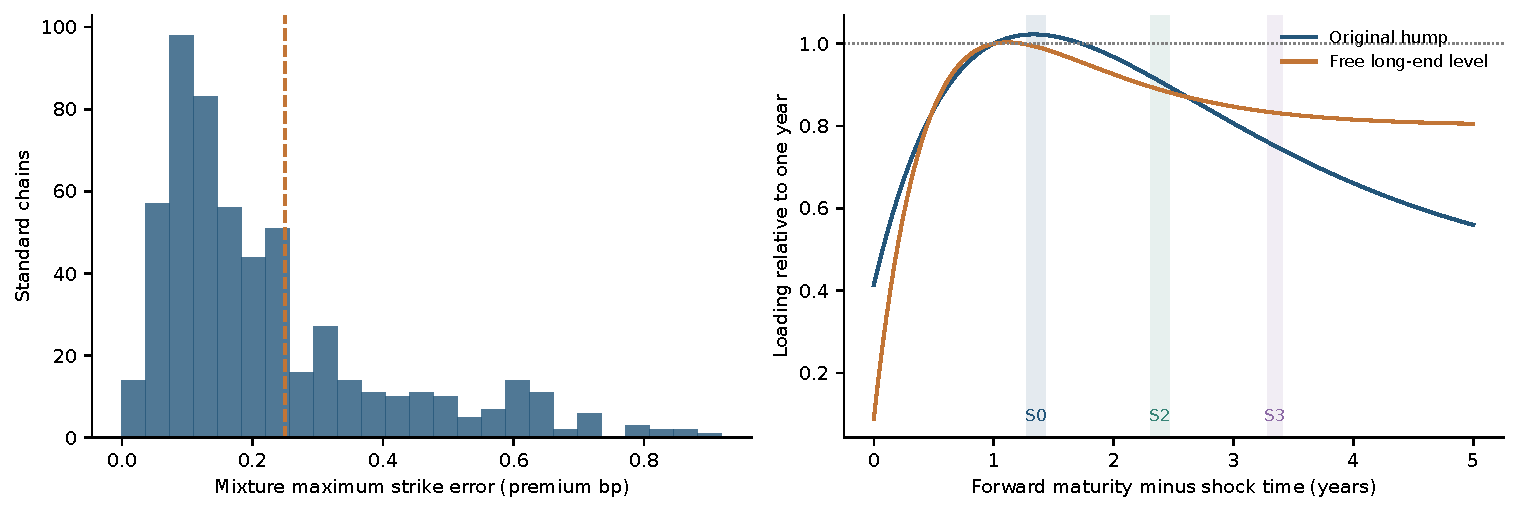
\includegraphics[width=\textwidth]{figures/empirical_extensions.pdf}
\caption{Extensions using the existing public settlements. Left: maximum selected-strike error in each standard chain's normal-mixture fit; the dashed line is 0.25 bp. Right: the two background loadings selected using standard, S0, and S2 observations, each divided by its value at one year. Shaded bands show the interquartile ranges of representative maturity distances $(a+b)/2-S/2$ for S0, S2, and S3. The exposure calculation integrates over the full accrual window and shock-time interval, not just these representative positions.}\label{fig:extensions}
\end{figure}

Each S3 exposure row lies in the span of its date's training rows, to numerical precision. Nonuniqueness of meeting allocations therefore does not alter the prediction conditional on the fitted training rows. These are point predictions, not bounds over price intervals. The new family was motivated by the earlier S3 errors; an untouched product or later sample is needed for independent validation of that family. Appendix~\ref{app:shapeprofile} retains the original-hump interval and shape-profile calculations, which show how shape uncertainty widens meeting-risk ranges.

\subsection{How large are exercise and mean adjustments?}\label{sec:exerciseempirical}
For an exercise benchmark, let the futures index be an arithmetic Brownian martingale with constant variance rate calibrated to the chain's fitted ATM variance. Discount at the constant rate reproducing its observed $D$. Value cash exercise on a recombining trinomial tree with 400, 800, and 1,600 time steps. Exercise is allowed at every step. Subtract the European value on the \emph{same} tree to isolate early exercise from terminal-payoff discretization. Appendix~\ref{app:empiricalmethod} specifies the tree and its pricing assumptions.

Use the first, middle, and last sample dates (30 March, 16 June, 14 September), and each chain's closest strike and two strike-band endpoints: 69 option observations. The 1,600-step exercise premium has median \textbf{0.023 bp} and maximum \textbf{0.377 bp}. The maximum change from 800 to 1,600 steps is 0.00050 bp; the largest European-tree error against the analytic normal price is 0.0034 bp. The largest exercise premium is for the 10 September 2027 expiry observed on 14 September 2026. Exercise is small for the median selected quote but material relative to a 0.25 bp allowance for some long expiries. It is too small in this benchmark to explain the multi-basis-point median midcurve error by itself. 

The mean effect can be sized without an exercise solver. Conditional on the 18 June ATM-proxy intervals at 1 bp, optimize the linear row $z/\delta$ in \eqref{eq:zrows}. For this sensitivity calculation only, insert those bp$^2$ allocations into the Gaussian model, converting variance to decimal units. The rate-mean displacement is
\[
F_0-\E^S[F_S]=\frac{G_0(1-e^{-z})}{\delta}.
\]
Across the three background specifications its compatible range is about $[0.00049,0.00096]$ rate bp for the first expiry and $[0.298,0.445]$ bp for the last, 11 June 2027. This is a conditional scale calculation, not a simultaneous fit of the exact cash means and variances. At fixed log variance, a European call or put price is Lipschitz in its rate mean with constant at most $D$. Hence the corresponding premium change is at most $D$ times the reported mean displacement. The longest expiries can require a wider allowance even when the smile interpolation itself is accurate.

We now widen the 18 June ATM-price allowances by both benchmark effects:
\begin{equation}\label{eq:robustallowance}
\varepsilon_\ell=0.25+\widehat{\mathrm{EEP}}_\ell
                         +D_\ell\overline{\Delta m}_\ell\quad\text{premium bp}.
\end{equation}
Here $\widehat{\mathrm{EEP}}_\ell$ is the 1,600-step exercise premium evaluated at the fitted ATM variance and zero moneyness. The mean bound $\overline{\Delta m}_\ell$ is the largest upper displacement across the three background specifications, each computed from its 1 bp seed intervals. This gives the same allowance for all three comparisons. The resulting allowances range from 0.253 to 0.989 bp across the seven expiries. Every allowance remains below 1 bp, so each new feasible set lies within the seed set used to bound its mean adjustment. The largest 800-to-1,600-step exercise change is 0.000033 bp.

\begin{table}[ht]
\centering\small
\begin{tabular}{lrr}
\toprule
Background & 16 September 2026 & 27 January 2027\\
\midrule
Constant & $[858,1100]$ & $[1910,2696]$\\
90-day cells & $[754,1384]$ & $[0,3560]$\\
Each expiry gap & $[0,1456]$ & $[0,3560]$\\
\bottomrule
\end{tabular}
\caption{18 June meeting-variance ranges in bp$^2$ with the expiry-specific allowances \eqref{eq:robustallowance}. Endpoints are rounded to the nearest bp$^2$.}\label{tab:robustranges}
\end{table}

The positive constant-background lower bounds survive (Table~\ref{tab:robustranges}). Relative to the 0.25 bp calculation, January's lower bound falls from 2,100 to 1,910 bp$^2$; allowing a flexible background still reduces it to zero. This establishes sensitivity to the background even after the specified exercise and mean allowances. The exercise estimate is a normal-model benchmark, not a uniform upper bound for every American model; the mean bound is conditional on inserting the proxy allocations into the Gaussian model.

\subsection{Does an ATM variance add across discrete meetings?}\label{sec:additivity}
A good smile interpolation does not guarantee an additive variance observation. For a centred terminal displacement $X$, the ATM proxy is $(\pi/2)(\E|X|)^2$. Independent Gaussian increments make it additive, but independent discrete increments generally do not. Consider equal-probability jumps of $\pm25$ bp. One jump and the sum of two such jumps both have $\E|X|=25$ bp, so both have ATM variance $625\pi/2=981.75$ bp$^2$, although their true variances are 625 and 1,250 bp$^2$. Adding two one-meeting ATM proxies overprices the two-meeting ATM call by 5.126 bp when the meetings are at $1/8$ and $2/8$ year and discounting is at 4\%.

Adding independent Gaussian background moderates the error but need not reduce it below 0.25 bp. With background volatility 50 bp per square-root year, eight equally spaced meetings produce a maximum ATM-price discrepancy of 2.323 bp from the additive one-increment proxy. If instead the additive schedule is allowed to fit each expiry exactly, its implied meeting variances range from 549 to 770 bp$^2$, despite all true meeting variances being 625 bp$^2$. The largest allocation errors occur at the first two meetings (770 and 549 bp$^2$); by the third, the inferred variance is 633 bp$^2$. In this example the error is concentrated where little background risk has accumulated, precisely the nearest meetings that front-end users often want to isolate. Appendix~\ref{app:additivity} gives the exact calculation and further background levels. The exercise-and-mean allowances above do not address this structural proxy error. The empirical ranges identify allocations within the additive ATM specification; interpreting them as variances of discrete policy outcomes requires a distributional pricing model or an additional sensitivity analysis.

Actual variance is additive across independent increments under a common measure, regardless of their distribution. As a companion check, Appendix~\ref{app:finalsensitivities} uses the fitted mixture second moments for the 18 June panel. This replaces the nonlinear ATM transform but introduces tail extrapolation. With the same ATM-scale perturbations and an additional 10\% moment allowance, constant-background September and January ranges are $[275,1058]$ and $[1549,4229]$ bp$^2$; both flexible backgrounds allow zero for both meetings. At 25\%, September's constant-background lower bound also vanishes and January's falls to 91 bp$^2$; at 50\%, both vanish. Without the additional allowance, constant and 90-day backgrounds are infeasible. Thus the background contrast appears under both proxies at a stated sensitivity level, but positive lower bounds are not robust to arbitrary tail uncertainty.
